\section{Suppressing systematic effects}
\def\secname{suppressing}\label{sec:\secname}

\noindent{\it Stephen Ridgway, Josh Myers, \ldots} % (Writing team)

Much of cosmology science may be limited by systematic errors rather than photon signal-to-noise.  

\subsection{Target Measurements}

It is expected that even after maximal optimization of camera optics and electronics, that systematic image shape errors will be associated with the orientation of the camera focal plane.  These can be partially reduced by randomization of the orientation of the camera with respect to the sky.  This is represented by the parameter RotSkyPos.  

Similarly, the telescope optics may harbor systematic aberrations, and these also could be mitigated by recording images with varying parallactic angle.  Another relevant parameter, RotTelPos, is indicative of the projected angle of the telescope optics on the sky.  

Uniformity of depth is essential - metrics and requirements will be added.


\subsection{Metrics}

A metric is available for RotSkyPos.  The metric computes, for any selected filter and simulation, a histogram of the distribution of rms values of RotSkyPos computed per field. It also computes basic statistics of these distributions.

\subsection{OpSim Analysis}


\begin{figure}
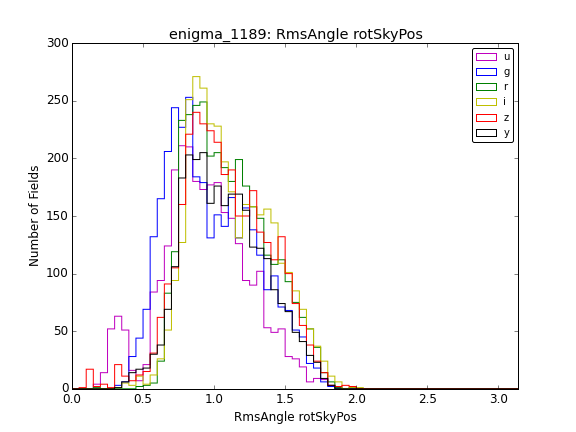
\includegraphics[width=5.0in]{enigma1189RmsAnglerotSkyPosugrizybandallpropsOPSIComboHistogram.png}
\caption{The relative angle of the detector plane with respect to the sky, RotSkyPos, as a histogram showing the number of fields vs. rms of the parameter.}
\label{RotSkyPos}
\end{figure}

The distribution of rms values by filter is shown in Figure \ref{RotSkyPos} for the current candidate baseline simulation, enigma\_1189.  As shown, the rms values cluster around the value 1 radian,  with typical values 1 +- 0.3 radian.  This compares to a completely uniform distribution over the half circle with an rms of 1.14.  

\subsection{Discussion}

The RotSkyPos metric analysis shows that the majority of fields have a good randomization of detector angles projected on the sky.

There are several limitations to this observation.

First, we do not have at present a quantitative requirement for randomization of this parameter.  In future development of weak lensing analysis, a criterion should be developed.

Second, a significant fraction of fields  have median values that are lower or higher than expected for a random distribution, with some far from uniformly distributed.  Regardless of the $per field$ criterion, it is desirable to avoid the incidence of individual discrepant fields.

The recommended criterion for randomization of RotSkyPos is not the behavior of the majority of the fields, but of the minority with the least random behavior.  The number of non-random fields should be minimized.  A recommended metric is the count of fields with median RMS less then 0.8 or greater than 1.5 radians (these values to be reviewed again as additional experience is gained with additional OpSim schedule simulations and weak lensing analysis.)

It is certain that actively controlling the statistics of RotSkyPos will require additional slewing of the camera rotator.  At present, the operations plan is to only slew when necessary to prepare for a filter change - that could be estimated at the equivalent of $\simeq 3$ complete rotations per day.  Figure \ref{RotSkyPos} shows that to render the distribution completely uniform would require moving all observing angles an average of $\simeq 30$ degrees, or 300 complete rotations per night.  The timing of this has not been considered.  Whether or not this uniformity could be achieved with less slew time if implemented in scheduling remains to be demonstrated.

A similar metric for RotTelPos should be developed. 